\section{Results and analysis}
\label{sec:results}

In this section we present the results of the three main topic areas of our study of PSB galaxies and their kinematical properties:

\begin{itemize}
    \item Basic property distributions
    \item Kinematic position angle analysis
    \item Radon transform profile classification and analysis
\end{itemize}

\subsection{Basic property distributions}
\label{sec:property-distributions}
Initially we performed some cursory checks on the distributions of some basic properties of our galaxy samples. Here we present those results as histograms comparing characteristic properties of CPSBs, RPSBs and their control galaxies. We show distributions of CPSB properties alongside those of the RPSB sample in terms of the following 3 fundamental properties: 
\begin{itemize}
\item stellar mass
\item redshift
\item S\'ersic index
\end{itemize}
The frequency distribution histograms of these properties are plotted in Figures \ref{fig:stellar-mass-plot}, \ref{fig:redshift-plot} and \ref{fig:Sersic-plot} respectively. The data underlying these  distributions is drawn from the MaNGA \texttt{drpAll} catalogue. The specific property values for each PSB is listed in Appendix \ref{sec:lists-of-psbs}, Tables \ref{tab:my-CPSBs} and \ref{tab:my-RPSBs}.

\textbf{Stellar mass:} The distribution in stellar mass for the CPSBs is compared to that of the RPSBs in Figure \ref{fig:stellar-mass-plot}. Both PSB groups span a similar range in mass. This result was noted previously during the interpretation of the colour-mass diagram depicted in Figure \ref{fig:Colour-Mass-PSBs}.

\begin{figure}
    \centering
    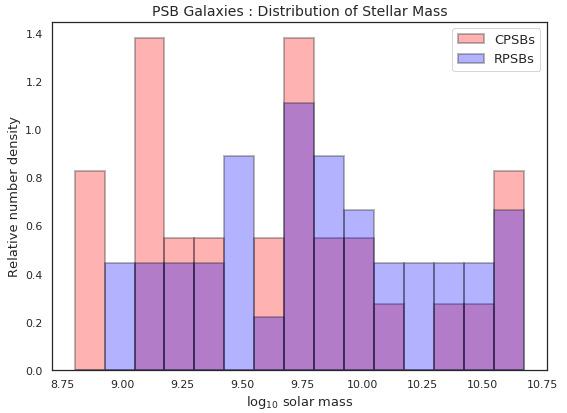
\includegraphics[width=\columnwidth]{images/JupyterPlots/Dist-Stellar-Mass-All.png}
    \caption[Distribution of stellar mass for CPSBs and RPSBs]{Distribution of stellar mass of our sample of CPSBs (red) and RPSBs (blue). On the logarithmic scale of $\log_{10}$\Msun\ a fairly uniform distribution of stellar mass is apparent for both populations, CPSBs and RPSBs.}
    \label{fig:stellar-mass-plot}
\end{figure}

\textbf{Redshift:} A comparison of the distribution in redshift for our CPSB and RPSB groups is shown in Figure \ref{fig:redshift-plot}. The redshift range of both groups lies in the range $0.01 < z < 0.08$. The shape of the redshift distribution of both groups is remarkably similar. We cannot distinguish the CPSB and RPSB populations based on redshift.

\begin{figure}
    \centering
    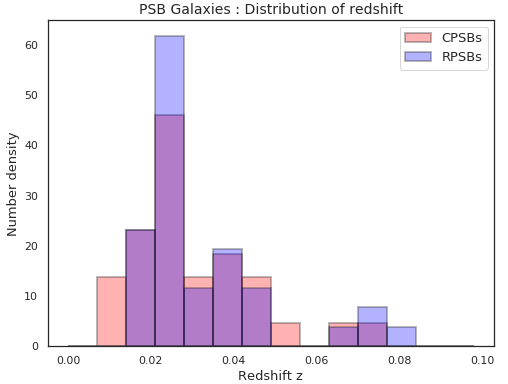
\includegraphics[width=\columnwidth]{images/JupyterPlots/Dist-z-All.png}
    \caption[PSB distribution in redshift]{Distribution in redshift z as obtained from the NSA.Z data value in the MaNGA \texttt{drpAll} file. The redshift distribution for the CPSB sample (shaded in red) is compared to that of the RPSB sample (blue).}
    \label{fig:redshift-plot}
\end{figure}

\textbf{S\'ersic index:} The surface brightness profile of a galaxy is generally a function of radius from the nucleus. The rate of change of brightness can be described by the S\'ersic function or S\'ersic index (SI). Low values of SI $\sim$1 relate to disc-type galaxies, whereas SI values of 3 or more are commonly measured in galaxies with compact bright nuclei indicative of more evolved systems. A wide range of S\'ersic index values is apparent in the distribution, as shown in Figure \ref{fig:Sersic-plot}, implying the presence of disparate morphologies in the sample. We note from the distribution that CPSBs tend to have higher S\'ersic index values than RPBs. This suggests that CPBs have more concentrated nuclei and a spheroidal morphology in contrast to the disc-like RPSBs with lower S\'ersic index values.

\begin{figure}
    \centering
    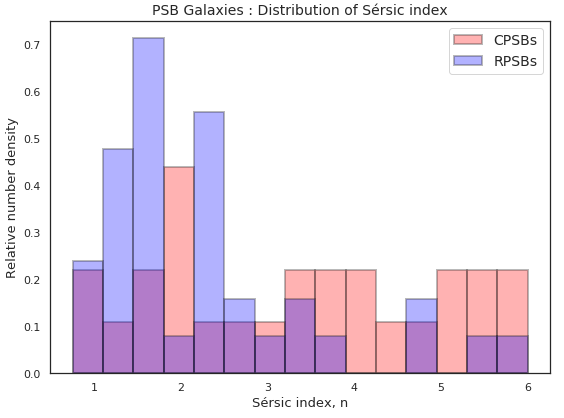
\includegraphics[width=\columnwidth]{images/JupyterPlots/Dist-Sersic-Index-All.png}
    \caption[Comparison of the distribution of S\'ersic index values of CPSBs and RPSBs]{Distribution of S\'ersic index (SI) values. The relative number density distribution of the S\'ersic index value for 26 CPSBs (red histogram) and 36 RPSBs (blue) are plotted. Five PSBs with unreliable SI values (SI = 6.000) in the NSA data  have been excluded.}
    \label{fig:Sersic-plot}
\end{figure}

In summary, the basic property distributions of CPSBs and RPSBs are very similar for stellar mass and redshift. The distribution of S\'ersic index does however reveal that RPSBs generally have lower SI values implying they are disc-like objects, while CPSBs with higher SI values indicate the morphology of spheroids.

%%%%====== Orphaned figures ======

\subsection{Kinematic position angle analysis}
\label{PA-misalignment}
The gas and velocity field position angle misalignment measurements for PSBs where the $\Delta$PA$_{k}$ \textgreater\ 30\textdegree\ are presented in Table \ref{tab:offsetCPSBs} for the CPSBs, and Table \ref{tab:offsetRPSBs} for the RPSBs. Here it can be seen that the number of PSBs having clearly defined $\Delta$PA$_{k}$ i.e. \textgreater\ 30\textdegree, is a small fraction of the PSB sample: 5 out of 30, or 17\% of CPSBs, and 9 out of 37, or 24\% of RPSBs. 

In contrast, looking at the control galaxies, the velocity field position angle variance of the CPSB and PSB control samples is shown in Figure \ref{fig:controlDeltaPAs}. Both sets of control galaxies have low values of velocity field $\Delta$PA$_{k}$, i.e. the stellar velocity and gas velocity fields are generally closely aligned.

\begin{table}
\centering
\caption{CPSBs with gas and stellar velocity kinematic PA offsets \textgreater 30\textdegree.}
\label{tab:offsetCPSBs}
\begin{tabular}{lccc}
\hline
PlateIFU  & Stellar PA & H$\alpha$ PA & $\Delta$PA \\
  & (deg.) & (deg.) & (deg.) \\
\hline
8313-6101 & 5 & 307 & 58 \\
8655-1902 & 335 & 127 & 152 \\
8725-1902 & 22 & 175 & 153 \\
8938-6102 & 214 & 47.5 & 166.5 \\
9494-3701 & 140.5 & 243 & 102.5 \\
\hline
\end{tabular}
\end{table}

\begin{table}
\centering
\caption[RPSBs with kinematic velocity PA offsets \textgreater 30\textdegree.]{RPSBs with gas and stellar velocity kinematic PA offsets \textgreater 30\textdegree.}
\label{tab:offsetRPSBs}
\begin{tabular}{lccc}
\hline
PlateIFU   & Stellar PA & H$\alpha$ PA & $\Delta$PA \\
  & (deg.) & (deg.) & (deg.) \\
\hline
8080-3704 & 24 & 154 & 130 \\
8262-3701 & 153.5 & 118.5 & 35 \\
8323-6103 & 109.5 & 313.5 & 156 \\
8439-6104 & 5.5 & 107 & 101.5 \\
8453-3704 & 44 & 91 & 47 \\
8486-1901 & 295.5 & 85 & 149.5 \\
8554-3701 & 250 & 68 & 178 \\
8932-12704 & 166.5 & 134.5 & 32 \\
9872-3701 & 208.5 & 81 & 127.5 \\
\hline
\end{tabular}
\end{table}

% \subsection{Distributions of kinematic position angles}
We now turn to analyse the distributions of the differential kinematic position angles $\Delta$PA$_{k}$ evident in our PSB samples and their control galaxies. Firstly, in Figure \ref{fig:deltaPAdistribution} we show the distribution of $\Delta$PA$_{k}$ in the CPSB sample versus the RPSB sample. This figure shows that CPSBs generally have higher $\Delta$PA$_{k}$ values than the RPSB population. This in an interesting finding in that CPSBs indicate a greater of misalignment between their gas and stellar velocity fields than RPSBs. If we consider past merger scenarios, this evidence may indicate that the masses of progenitor components are comparable in the CPSB distribution, but less so in the case of RPSB mergers.

\begin{figure}
    \centering
    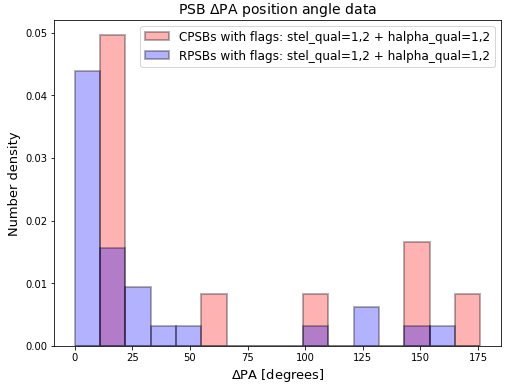
\includegraphics[width=\columnwidth]{images/JupyterPlots/Dist-Delta-PA-All-GoodFlags.png}
    \caption[Distribution of PSB stellar and gas velocity field position angles]{Distribution of PSB galaxy velocity field position separation angles ($\Delta$PA$_{k}$) for those PSBs with stellar velocity and gas velocity characteristics flagged as 'good' as denoted in the legend (see the text in Section \ref{sec:kinemetry-analysis-method-description} for details). CPSB $\Delta$PA$_{k}$ density weights are plotted in red, RPSB $\Delta$PA$_{k}$ weights in blue.}
    \label{fig:deltaPAdistribution}
\end{figure}

We now examine the distribution in kinematic position angle of the subject PSB groups: CPSBs, RPSBs and their respective control galaxy samples. The distribution in $\Delta$PA$_{k}$ of the CPSB sample against their control population is shown in Figure \ref{fig:CPSBvsControlDeltaPAs}. The CPSBs have significantly larger kinematic $\Delta$PA$_{k}$ than the control galaxy group.

\begin{figure}
    \centering
    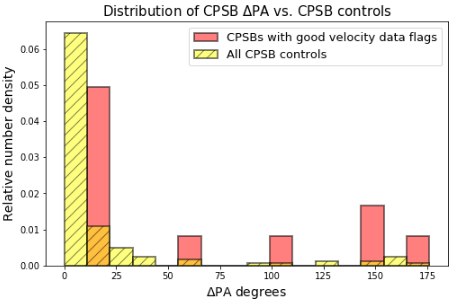
\includegraphics[width=\columnwidth]{images/JupyterPlots/DIST-DPA-CPSB+FLAGS+controls.png}
    \caption[Distribution of CPSB $\Delta$PA vs. their CPSB controls]{Distribution of CPSB stellar and gas velocity position angle difference $\Delta$PA vs. their CPSB controls. Note the CPSBs selected are a subset where their gas and stellar kinematic map data has been flagged as usable. CPSBs PA distributions are plotted in red with their CPSB controls in yellow with hatching. The PA offset in CPSB $\Delta$PA is discussed in the text.}
    \label{fig:CPSBvsControlDeltaPAs}
\end{figure}

The distribution in kinematic position angle of the RPSB sample against their control population is shown in Figure \ref{fig:RPSBvsControlDeltaPAs}. The RPSBs possess larger kinematic $\Delta$PA$_{k}$ than their control galaxy group, but to a lesser extent than the CPSBs to their controls. Significantly, we see an emerging trend: CPSBs exhibit larger kinematic $\Delta$PA$_{k}$ than the RPSB group.

To complete the picture, we look at the comparative distribution of the control galaxy $\Delta$PA$_{k}$ for both PSB groups: CPSBs and RPSBs. This is shown in Figure \ref{fig:controlDeltaPAs}. We note that the distributions of control galaxy $\Delta$PA$_{k}$ are very similar and bunched at less than 20\textdegree. 

\begin{figure}
    \centering
    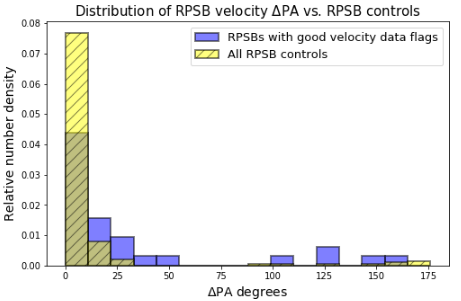
\includegraphics[width=\columnwidth]{images/JupyterPlots/DIST-Good-RPSB+Flags+Controls.png}
    \caption[Distribution of RPSB velocity $\Delta$PA vs. their RPSB controls]{Distribution of RPSB stellar and gas velocity $\Delta$PA vs. their RPSB controls. Note the RPSBs selected are a subset where their gas and stellar kinematic map data has been flagged as usable. RPSB PA distributions are plotted in blue with their RPSB controls in yellow with hatching}
    \label{fig:RPSBvsControlDeltaPAs}
\end{figure}


\begin{figure}
    \centering
    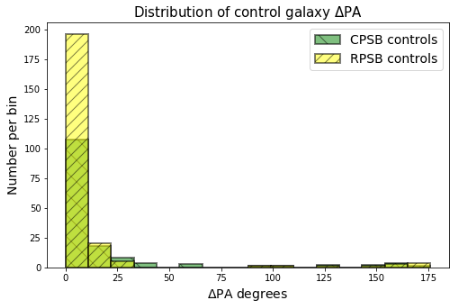
\includegraphics[width=\columnwidth]{images/JupyterPlots/DIST-Control-DPA-both.png}
    \caption[Distribution of control galaxy $\Delta$PA$_{k}$]{Distribution of both CPSB and RPSB control galaxy stellar and gas velocity field position angle difference $\Delta$PA$_{k}$. CPSB control galaxy distributions are plotted in green, RPSB control galaxy distributions in yellow with hatching.}
    \label{fig:controlDeltaPAs}
\end{figure}

\subsection{Statistical tests of kinematic position angle distributions}
\label{sec:K-S-test}
In order to investigate the likelihood that the difference in kinematic position angles, $\Delta$PA$_{k}$, of CPSBs, RPSBs, and their respective control galaxy groups are drawn from the same underlying population we employed a \textbf{Kolmogorov-Smirnov test} (K-S test) analysis. The K-S test is a statistical analysis designed to determine if two samples come from the same underlying distribution, see e.g. \citet{hodges1958significance}. We implement this test using the Python SciPy package \texttt{scipy.stats.kstest} module\footnote{\href{https://docs.scipy.org/doc/scipy/reference/generated/scipy.stats.ks\_2samp.html}{https://docs.scipy.org/doc/scipy/reference/generated/scipy.stats.ks\_2samp.html}}. This Python implementation accepts samples of different size which suits our purpose here.

We ran the two-sided K-S test statistic on the distribution of $\Delta$PA$_{k}$ kinematic position angle analysis described in Section \ref{sec:kinemetry-analysis-method-description}. The results of the K-S test are presented in Table \ref{tab:K-S-tests}. The statistical significance inferred from the from the K-S test is that a high value of the test statistic, typically > 0.1, together with a low p-value, < 10$^{-2}$ indicates that the samples are drawn from different statistical distributions. The K-S test results show that  that position angle differences, $\Delta$PA$_{k}$, of the CPSB and RPSB groups show that they originate from different distributions. Also the $\Delta$PA$_{k}$ of each PSB group is from a different distribution than its corresponding control galaxy sample. These results are important in that they reveal statistically significant differences in the kinematic properties of the CPSB group with large $\Delta$PA$_{k}$, the RPSB group with intermediate $\Delta$PA$_{k}$ and the control galaxy groups which exhibit small $\Delta$PA$_{k}$. 

\begin{table}
\caption[Kolmogorov-Smirnov statistical test of $\Delta$PA distributions]{Result of a Kolmogorov-Smirnov statistical test performed on $\Delta$PA$_{k}$ distributions from the CPSB, RPSB and control galaxy samples. A high value of the K-S statistic \textgreater 10\%, together with a low p-value, \textless 1\% indicates that the samples originate from different statistical distributions.}
\label{tab:K-S-tests}
\begin{tabular}{llcc}
\hline
$\Delta$PA sample 1  & $\Delta$PA sample 2 & K-S statistic & p-value \\
\hline
CPSB & RPSB & 0.467 & 4.0$\times10^{-2}$ \\
CPSB & CPSB controls & 0.755 & 5.3$\times10^{-6}$ \\
RPSB & RPSB controls & 0.520 & 5.1$\times10^{-7}$ \\
CPSB controls & RPSB controls & 0.197 & 1.3$\times10^{-3}$ \\
\hline
\end{tabular}
\end{table}

\subsection{Radon profile classification}
\label{sec:Radon-profile-classification}

A summary of the results of the visual classification method is presented in Table \ref{tab:Radon-class-summary}.  A few galaxies could not be visually classified (NC) because of masked areas in the central spaxels of the MaNGA stellar velocity maps, or low S/N regions. These deficiencies prevented the Radon transform code from providing sufficient trace profile data points to enable visual classification. The results of the Radon profile classification process for each of the individual target galaxies is provided in Appendix \ref{sec:visual-classification-tables}, Table \ref{tab:full-visual-classification}. 

\begin{table}
    \centering
    \caption[Summary of Radon profile type visual classifications]{Summary of the classification of Radon profile types as categorised visually in the CPSB and RPSB groups and their control samples.}
    \label{tab:Radon-class-summary}
    \begin{tabular}{lc}
    \hline
    Radon profile type & Number in classification \\
    \hline
    Type-A: Asymmetric & 25 \\
    Type-C: Constant & 38 \\
    Type-IB: Inner Bend & 22 \\
    Type-OB: Outer Bend & 17 \\
    Type-OB+IB: Outer and Inner Bends & 17 \\
    NC: Not classified & 8 \\
    \hline
    \end{tabular}
\end{table}

On completion of the Radon profile classification exercise we investigated the distribution of the Radon profile types in each of the PSB categories (CPSB and RPSB) and their control samples (CPSB-controls and RPSB-controls). As described in Section \ref{sec:Radon-classification} the visual classification assessment was performed on the appearance of the Radon output plots: the Radon Transform (RT), Radon profile trace and stellar velocity map (see Figure \ref{fig:8442-3704-complete} for an example of this output), without prior knowledge of the PSB group category (CPSBs, RPSBs or controls). A summary of the Radon profile visual classification assessments obtained by Classifier A is provided in Table \ref{tab:Radon-VC-results}. These results reveal that galaxies exhibiting Radon transform profile bend features: Type-IB, Type-OB and Type-IB+OB, are more prevalent in CPSBs (16 out of 27, or 59\% of galaxies classified) than in RPSBs (15 out of 36, or 42\% of those classified). A similar trend is found in the control groups. Bend-type features are found in 18 out of 29, or 62\% of CPSB controls, while 11 out of 31, or 35\% of RPSB controls display bend-type features. These results are portrayed graphically as a grouped bar graph in Figure \ref{fig:Radon-grouped-barchart}.

\begin{table*}
\caption[Radon profile visual classification CPSB and RPSB samples and their control galaxies - classifier A]{Results of the Radon profile visual classification assessments for CPSB and RPSB samples and their control galaxies obtained from classifier A. PSBs and controls were assigned a Radon profile according to the appearance of the shape of the Radon profile trace plot. Where clear features were evident the galaxy was assigned a Radon profile Type as described in the text. Galaxies that could not be objectively classified due to poor data were flagged as 'not classified' (NC). The percentage of each Type of those classified in the group shown in parentheses.}
\label{tab:Radon-VC-results}
\begin{tabular}{lccccccc}
\hline
 & \begin{tabular}[c]{@{}c@{}}Classified \end{tabular} & Constant & Inner Bend & Outer Bend & \begin{tabular}[c]{@{}c@{}}Inner Bend + \\ Outer Bend\end{tabular} & Asymmetric & \begin{tabular}[c]{@{}c@{}}Not\\ Classified\end{tabular} \\
Galaxy group &  & (Type-C) & (Type-IB) & (Type-OB) & (Type-IB+OB) & (Type-A) & (NC) \\
 \hline
CPSBs & 27 & 7 (26\%) & 6 (22\%) & 5 (19\%) & 5 (19\%) & 4 (15\%) & 1 \\
CPSB controls & 29 & 6 (21\%) & 7 (21\%) & 6 (21\%) & 5 (17\%) & 5 (17\%) & 2 \\
RPSBs & 36 & 14 (39\%) & 5 (14\%) & 5 (14\%) & 5 (14\%) & 7 (19\%) & - \\
RPSB controls & 31 & 10 (32\%) & 4 (13\%) & 3 (10\%) & 4 (13\%) & 10 (32\%) & 5 \\
\hline
Totals & 123 & \multicolumn{1}{l}{37 (30\%)} & 22 (18\%) & 19 (15\%) & 19 (15\%) & 26 (21\%) & 8 \\
\hline
\end{tabular}
\end{table*}

\begin{figure}
    \centering
    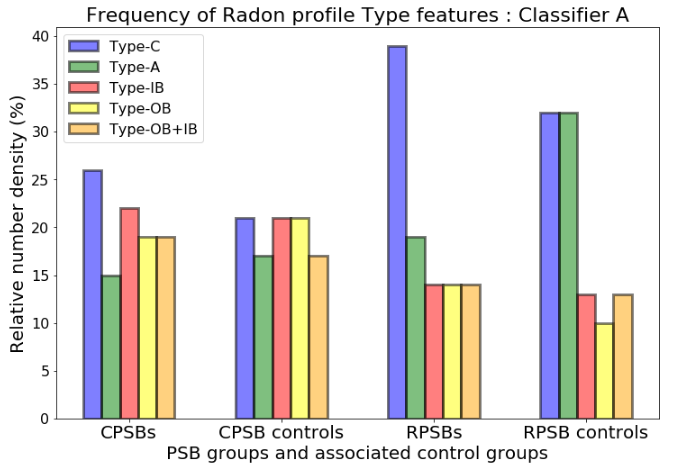
\includegraphics[width=\columnwidth]{images/JupyterPlots/PROFILE-GROUPS-CLASSIFIER-A.png}
    \caption[Radon profile Type classifications determined by classifier A]{The results of the Radon profile visual classification exercise obtained by classifier A is shown for the 4 galaxy groups of interest: CPSBs, CPSB controls, RPSBs and their controls. The numerical frequency of each of the 5 Radon profile type features from Table \ref{tab:Radon-VC-results} are displayed in this grouped bar plot. The colour coding of each type feature is shown in the legend.}
    \label{fig:Radon-grouped-barchart}
\end{figure}

\begin{table}
\centering
\caption{CPSBs with PA offset \textgreater 30\textdegree\ matched with their visually determined Radon profile Type.}
\label{tab:offsetCPSBs-Radon-Type}
\begin{tabular}{lcccc}
\hline
PlateIFU  & Stellar PA & H$\alpha$ PA & $\Delta$PA & Radon profile\\
  & (deg.) & (deg.) & (deg.) & Type \\
\hline
8313-6101 & 5 & 307 & 58 & OB \\
8655-1902 & 335 & 127 & 152 & OB+IB \\
8725-1902 & 22 & 175 & 153 & OB+IB \\
8938-6102 & 214 & 47.5 & 166.5 & C \\
9494-3701 & 140.5 & 243 & 102.5 & C \\
\hline
\end{tabular}
\end{table}

\begin{table}
\centering
\caption[RPSBs with PA offset \textgreater 30\textdegree\ matched with their visually determined Radon profile Type]{Similar to Table \ref{tab:offsetCPSBs-Radon-Type}. RPSBs with PA offset \textgreater 30\textdegree\ matched with their visually determined Radon profile Type.}
\label{tab:offsetRPSBs-Radon-Type}
\begin{tabular}{lcccc}
\hline
PlateIFU   & Stellar PA & H$\alpha$ PA & $\Delta$PA & Radon profile \\
  & (deg.) & (deg.) & (deg.) & Type\\
\hline
8080-3704 & 24 & 154 & 130 & C \\
8262-3701 & 153.5 & 118.5 & 35 & C \\
8323-6103 & 109.5 & 313.5 & 156 & C \\
8439-6104 & 5.5 & 107 & 101.5 & A \\
8453-3704 & 44 & 91 & 47 & C \\
8486-1901 & 295.5 & 85 & 149.5 & C \\
8554-3701 & 250 & 68 & 178 & OB \\
8932-12704 & 166.5 & 134.5 & 32 & A \\
9872-3701 & 208.5 & 81 & 127.5 & OB+IB \\
\hline
\end{tabular}
\end{table}

It is noted the majority of PSBs with $\Delta$PA offsets \textgreater 30\textdegree\ listed in Tables \ref{tab:offsetCPSBs-Radon-Type} and \ref{tab:offsetRPSBs-Radon-Type} show constant or asymmetric radial Radon profiles, however a few outer and inner bend profiles are evident. 

% \subsection{Independent visual classification}
\label{independent-classification}
An independent Radon profile classification exercise was carried out by a second classifier, Classifier B, following the same procedure as described in Section \ref{sec:Radon-classification}. The results of this supplementary classification are summarised in Table \ref{tab:Radon-VC2-results}, and displayed graphically in Figure \ref{fig:Radon-grouped-barchart-B}. The results obtained by Classifier B can be compared with and contrasted to the results obtained by Classifier A, as presented earlier in Table \ref{tab:Radon-VC-results} and Figure \ref{fig:Radon-grouped-barchart}.

\begin{table*}
\caption[Radon profile visual classification CPSB and RPSB samples and their control galaxies - classifier B]{Results of the supplementary Radon profile visual classification assessments for CPSB and RPSB samples and their control galaxies. The information presented is as per Table  \ref{tab:Radon-VC-results} but provides the profile classification results visually assessed by independent classifier B.}
\label{tab:Radon-VC2-results}
\begin{tabular}{lccccccc}
\hline
 & \begin{tabular}[c]{@{}c@{}}Classified \end{tabular} & Constant & Inner Bend & Outer Bend & \begin{tabular}[c]{@{}c@{}}Inner Bend + \\ Outer Bend\end{tabular} & Asymmetric & \begin{tabular}[c]{@{}c@{}}Not\\ Classified\end{tabular} \\
Galaxy group &  & (Type-C) & (Type-IB) & (Type-OB) & (Type-IB+OB) & (Type-A) & (NC) \\
 \hline
CPSBs & 28 & 1 (4\%) & 4 (14\%) & 5 (18\%) & 5 (18\%) & 13 (46\%) & - \\
CPSB controls & 29 & 2 (7\%) & 3 (10\%) & 1 (3\%) & 5 (17\%) & 18 (62\%) & 1 \\
RPSBs & 36 & 1 (3\%) & 6 (17\%) & 7 (19\%) & 5 (14\%) & 17 (47\%) & - \\
RPSB controls & 34 & 0 (0\%) & 4 (11\%) & 4 (11\%) & 7 (19\%) & 19 (53\%) & 2 \\
\hline
Totals & 127 & \multicolumn{1}{l}{ 4 (3\%)} & 17 (13\%) & 17 (13\%) & 22 (17\%) & 67 (53\%) & 3 \\
\hline
\end{tabular}
\end{table*}


\begin{figure}
    \centering
    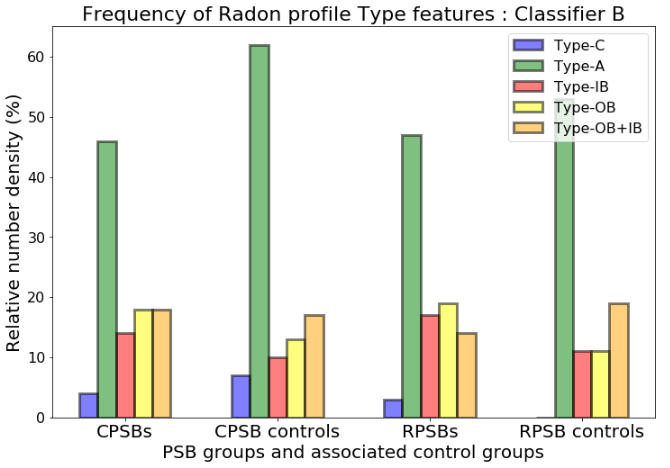
\includegraphics[width=\columnwidth]{images/JupyterPlots/PROFILE-TYPES-CLASSIFIER-B.png}
    \caption[Radon profile Type classifications determined by Classifier B]{The results of the Radon profile visual classification exercise obtained by Classifier B is shown for the 4 galaxy groups of interest: CPSBs, CPSB controls, RPSBs and their controls. The numerical frequency of each of the 5 Radon profile type features from Table \ref{tab:Radon-VC2-results} are presented graphically in this grouped bar plot. The colour coding of each type feature is shown in the legend.}
    \label{fig:Radon-grouped-barchart-B}
\end{figure}

We note a significant disparity in the the numbers classified in each of the Type categories as determined by Classifiers A and B. The disparity is particularly noticeable for the categorisation of Type-C (constant) and Type-A (asymmetric) profiles. This imbalance may be due to the similarity of the guideline examples given in Figure 7 of \cite{2018MNRAS.480.2217S}. Both the example profiles display some measure of asymmetry and also show a relatively constant profile in their central regions, around radius $\rho = 0$. In fact there is some indication of inner bend features in both the Type-C and Type-A examples. Evidently visual classification is difficult, and this comment was made by both classifiers. We continue further discussion on this point in Section \ref{sec:discussion}. Setting aside the difficulties of Type-A and Type-C classifications, we note that similar numbers galaxies with with bend-type features, Type-OB, Type-IB and Type-OB+IB were identified by both classifiers. We emphasise, however, that there was still considerable variation in classification for specific individual galaxies. The results of the two independent classifications (Classifiers A and B) for the 3 bend-feature categories, in each of the 4 galaxy groups, are summarised in Table \ref{tab:Radon-VC3-results}. There is little to infer from these results, maybe only that both classifiers determined similar numbers of Types in each galaxy category. This similarity is strongly contradicted, however, by the classifications determined by Classifiers A and B for specific galaxies. This can be seen by comparing the Type classification listings of Tables \ref{tab:full-visual-classification} and \ref{tab:visual-classification-B} in Appendix \ref{sec:visual-classification-tables}.

\begin{table*}
\caption[Comparison of Radon profile classifications by classifiers A and B, excluding Types A and B]{Comparison of Radon profile Type classifications provided by Classifiers A and B, excluding Type-C and Type-A profiles.}
\label{tab:Radon-VC3-results}
\begin{tabular}{lccccccccc}
\hline
 & \multicolumn{3}{c}{Classifier A} & \multicolumn{3}{c}{Classifier B} \\ 
Group & Type-IB & Type-OB & Type-IB+OB & \multicolumn{1}{l}{Type-IB} & \multicolumn{1}{l}{Type-OB} & \multicolumn{1}{l}{Type-IB+OB} \\
\hline
CPSBs & 6 & 5 & 5 & 4 & 5 & 5 \\
CPSB controls & 7 & 6 & 5 & 3 & 1 & 5 \\
RPSBs & 5 & 5 & 5 & 6 & 7 & 5 \\
RPSB controls & 4 & 3 & 4 & 4 & 4 & 7 \\
\hline
Totals & 22 & 19 & 19 & 17 & 17 & 22 \\
\hline
\end{tabular}
\end{table*}

